\section{Final Implementation}\label{chap:afm-cs-final}

This chapter is a story of rising tides and all ships being lifted. I wish to give raster scanning a fair shake\footnote{It would not be hard to argue that I have failed in that endevour. Because the $X$-axis control scheme is designed for tracking step-inputs, it has more damping and lower bandwidth than what one could probably achieve if only raster scanning.}. Therefore, where appropriate, the improvements made to CS scanning are also applied to raster scanning. This means that both raster and CS scanning use the state space compensator designed in Chapter~\ref{chap:mpc_slf} and the $Z$-axis controller designed in Chapter~\ref{chap:zaxis-improv}.
This improves the results for both methods, compared to Chapter~\ref{chap:cs_init}. 

 The first section discusses several modifications (i.e., differences to Chapter~\ref{chap:cs_init}) to the CS-scanning cycle. Section \ref{sec:post_process} discusses the post-processing techniques used. Section \ref{sec:rdi} develops a new metric to compare the relative damage done by different scans and Section~\ref{sec:psnr_ssim_limits} takes a closer look at the SSIM and PSNR metrics in an effort to understand what ''reasonable'' numbers look like for AFM images taken with our AFM. Similarly, Section~\ref{sec:cs_sim} looks at some CS simulations (based on real raster scans) to help us understand what, ideally, we should see from the experiments performed in Section~\ref{sec:results:final}. 

\section{The Modified CS-Cycle}\label{sec:modfied_cs_cycle}
The final implementation is similar to the initial implementation originally described in Chapter~\ref{chap:cs_init}. However, there are some differences. These are summarized in
Table~\ref{tab:cs_cycle_diff}
\begin{table}
  \centering
  \caption{Summary of the differences between the initial CS implementation and the final version.}
  \label{tab:cs_cycle_diff}
  \begin{tabular}{c|p{1.75in}|p{1.75in}}
    state &  initial implementation & current implementation \\
    \hline
    $XY$-move & control: PI     & control: LQG           \\
    \hline
    tip-settle & $XY$ does not move & $XY$ starts scanning  (pre-scan)\\
    \hline
    $\mu$-path scan & finish with post-scan & no post scan \\
    \hline
    tip-up & $Z$-axis feedback off. Set ${u_k=u_{\textrm{up}}}$. & $Z$-axis feedback on. Set ${r_Z=r_{Z,\textrm{up}}}$. Implement anti-windup. \\
  \end{tabular}
\end{table}
The new state machine is diagramed in Fig.~\ref{fig:sm_final}. 
The primary modifications are (i) a pre-scan during $Z$-axis settling period, (ii) not intentionally disengaging during tip-retraction; (iii) at the end of a scan, return to state-0, so that everything remains in closed-loop.

Several cycles of the modified scheme are shown in Fig.~\ref{fig:cs_cycle_final}. Each of these differences is discussed more fully in the following three subsections.
\begin{figure}[ht!]
  \centering
  \includesvg[scale=0.85]{plots-afm-cs-final/figures/cs_cycle.svg}
  \caption{Several CS cycles. Each state is indicated by color.}
  \label{fig:cs_cycle_final}
\end{figure}

\begin{figure}
  \centering
    \includesvg[width=.9\textwidth]{plots-afm-cs-final/figures/state-machine-final.svg}
    \caption{Diagram of the state-machine implemented in the final design.}
    \label{fig:sm_final}
\end{figure}

\subsection{Cantilever does not need to fully disengage.}
In the initial implementation, we insisted that the during tip-retraction (state-5), the cantilever tip should fully break contact with the surface. Here, we impose no such requirement. Rather, we change the $Z$-setpoint during tip-retraction to only pull away far enough that the deflection signal stays low (i.e., below the scanning setpoint), even while we run across the surface.

\textbf{Motivation} The motivation for this is two-fold. First, there is the obvious advantage that, by not pulling the tip so away, there is less distance to recover during the re-engagement. The original idea was to pull away from the surface far enough to disengage, then step back down towards the surface by some fraction of the step up. This proved impractical for several reasons. First, it requires the control system to be able to detect when disengagement has occurred. While preliminary experiments indicate it may be possible to achieve this by detecting a change in the derivative of the deflection signal, the actual value of the control signal which achieved dis-engagement proved to be highly variable (ranging from about 0.6 v to over 3 volts (210 nanometers to over a micron)) and sometimes saturating the control signal without disengagement. Experiments indicate that the dis-engagement point depends on (at least) the tip condition and the cantilever spring constant \footnote{The numbers cited used a cantilever with $k\approx .1$~N/m. Experiments using a cantilever with $k\approx 50$ N/m yielded much more consistent and much smaller needed dis-engagement control signals. However, cantilevers with such large spring constants are tapping-mode cantilevers, a mode which our AFM is incapable of. Scanning in contact mode with such a cantilever implies that a very large force is being applied to the sample.}.

Such large pull-away distances are problematic, especially for our AFM, which lacks a $Z$-position sensor. The difficulty is that when the tip is re-engaged with the sample from far away, this incites a large drift transient.
This is shown in Fig.~\ref{fig:z_drift} under the panels labeled ``big lift''.
By starting the re-engagement closer to the sample, this transient is much smaller. Without a $Z$-position sensor, we have to let this drift die out or it will corrupt the image. Thus, even if the step-up-down scheme could be made to work, the overall time would still be limited by this drift. I made some effort to fit an LTI model to the drift mode, so this affect could be removed in post-processing. Unfortunately, as we saw in Section~\ref{sec:modeling_remaining}, an LTI drift model does not adequately describe the drift transient, because the drift rate seems to depend on the control history.

A third advantage is that, given the \emph{same} absolute starting height above the specimen, re-engagement is faster when the tip has not snapped free. The reason for this is that when the cantilever snaps away from the specimen surface, the deflection signal is essentially saturated. This gives the control loop an artificially small error signal, which leads to a very sluggish descent.


\textbf{Justification} Ultimately the concern is damage to the sample and tip, which is caused by the force imparted by the cantilever probe \cite{clayton_review_2009}. The deflection signal, though un-calibrated (meaning it does not directly lead to a value in $kN$), is proportional to that force, because it is proportional to how much the cantilever is bent. I.e., a large (towards $+\infty$) deflection implies the spring force of the cantilever is pushing hard into the sample, thereby inducing damage. In a typical imaging scenario, we choose a deflection setpoint, (say $0.15$~[v], as in Fig.~\ref{fig:z_drift}), and have in some way decided that this is sufficient, all else being equal, to not damage things too much.

Thus, rather than completely dis-engaging the tip from the surface, I propose to simply move the setpoint towards $-\infty$ during the $XY$-move. If this new setpoint is sufficiently far away, the deflection signal will stay below the scanning setpoint, which we had decided was a ''safe'' value. The change in setpoints is achieved via the multiplexer in Fig.~\ref{fig:afm_bd_dinv_final} which selects either the scanning setpoint $r_{Z,s}$ or the retraction setpoint $r_{Z,\textrm{up}}$ based the current state.
\begin{figure}[t]
  \centering
  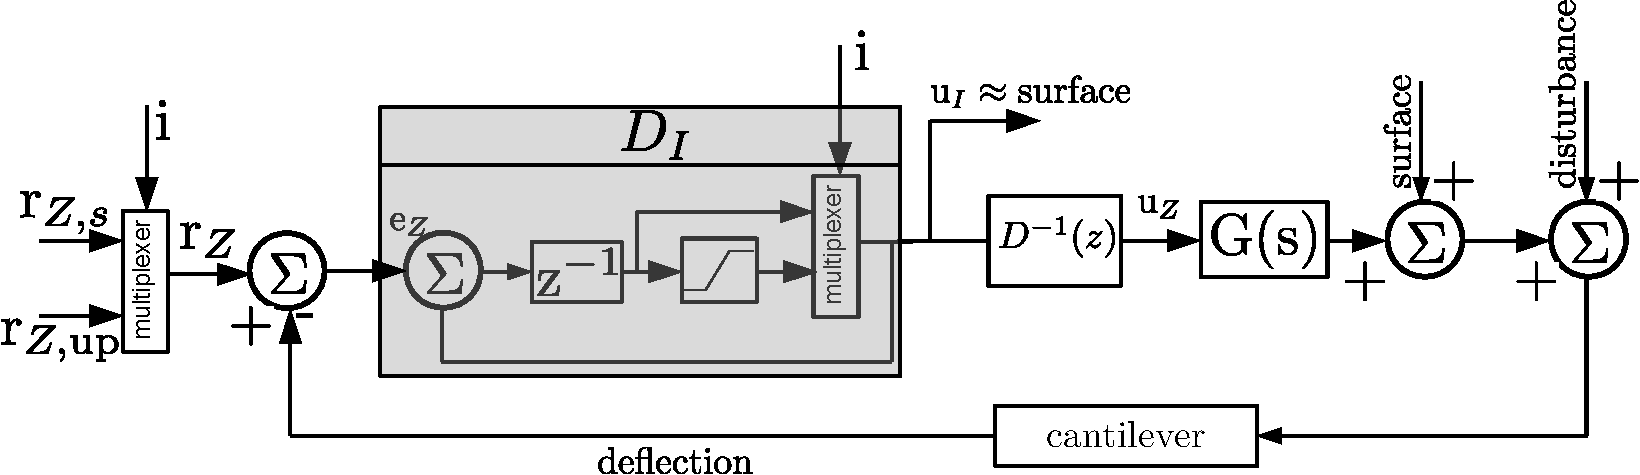
\includegraphics[width=0.75\textwidth]{plots-afm-cs-final/figures/AFM_loop_Dinv_antiwup-crop.pdf}
  \caption{Block diagram of the $Z$-axis control loop. The anti-windup is active for decision index $i\in\{0,1,5\}$, which correspond to states such that $r_Z=r_{Z,\textrm{up}}$.}
  \label{fig:afm_bd_dinv_final}
\end{figure}

\begin{figure}[ht!]
  \begin{subfigure}{.48\textwidth}
    \includesvg[width=1\textwidth]{plots-afm-cs-final/figures/justify_small_lift.svg}
    \caption{ }
    % \label{fig: }
  \end{subfigure}
  \begin{subfigure}{.48\textwidth}
    \includesvg[width=01\textwidth]{plots-afm-cs-final/figures/justify_small_lift_zoom.svg}
    \caption{ }
    % \label{fig: }
  \end{subfigure}
  \caption{One CS-cycle with different dis-engagement heights. (a) Full view. (b) Zoomed-in view. Note the  drift transient in the left panel of (b). }
  \label{fig:z_drift}
\end{figure}

This new scheme does not imply that the cantilever \emph{never} fully disengages. Occasionally, the new setpoint is far enough away that the probe does still snap away from the sample surface. 
When this happens, the integrator, $D_I(z)$, will windup. This happens because typically, the desired setpoint $r_{Z,\textrm{up}}$ is more negative than the free (disengaged) value of the deflection. Thus, the sensor signal is essentially saturated and no matter how far the $Z$-actuator tries to move, no change will result in the deflection, leading to windup and a control signal that exceeds the actuator bounds. To deal with this, we implement an anti-windup scheme for all states where $r_Z=r_{Z,\textrm{up}}$, i.e., states (0), (1) and (5). This is illustrated in the block diagram in Fig.~\ref{sec:modfied_cs_cycle}. During these states, the output of the accumulator is saturated before its own internal feedback. 

\subsection{The pre-scan}
\begin{figure}
  \begin{subfigure}{.33\textwidth}
    \includesvg[width=1\textwidth]{plots-afm-cs-final/figures/zbounce_uz_example.svg}
    \caption{ }
    \label{fig: }
  \end{subfigure}
  \begin{subfigure}{.33\textwidth}
     \includesvg[width=1\textwidth]{plots-afm-cs-final/figures/prescan_uz_example.svg}
    \caption{ }
    \label{fig:uz_prescan}
  \end{subfigure}
  \begin{subfigure}{.33\textwidth}
     \includesvg[width=1\textwidth]{plots-afm-cs-final/figures/prescan_zbounce_PSD.svg}
    \caption{ }
    \label{fig: }
  \end{subfigure}
  \caption{(a) A ``$Z$-bounce'' experiment where the $XY$-stage is motionless and the cantilever is repeatedly engaged and disengaged. (b) One cycle of a tightly packed set of CS-cycles where the movement between each measurement location is 0. (c) PSDs from the portions of the trajectories which are colored blue and turquoise, averaged over many such cycles, demonstrating that the scan process itself reduces vibration in the $Z$-axis.}
  \label{fig:prescan_difference}
\end{figure}
After the tip-descent, we begin scanning in a ``pre-scan'' phase (state (3)). To motivate, this consider Fig.~\ref{fig:prescan_difference}. The left panel represents what we call a ``$Z$''-bounce experiment, where the $XY$-stage stays motionless, but we repeatedly retract and re-engage the tip with specimen, exactly as we would in a CS scan. The right panel represents a single cycle from specialized CS pattern, where the $\mu$-paths are still 500 nm long, but the paths are separated by 0 pixels. In this case, the specimen is freshly cleaved mica. The goal here is to eliminate (i) any oscillations which arise from the $XY$-move (which, as we will show in Section ~\ref{sec:need_mimo}, can be significant) and (ii) to have a perfectly flat surface to scan over so that there are as few disturbances as possible entering the control loop. Finally, the middle panel of Fig.~\ref{fig:prescan_difference} shows the PSDs of the left and right panels (but averaged over many similar cycles). Note that the PSD is only computed from the combination of the blue and turquoise signals.

What we see then, is that, for some unknown (to me) reason, scanning reduces the amount of energy that shows up near 215 Hz. The idea behind the pre-scan is to take advantage of this.
The pre-scan phase is relatively long (150 samples), especially for the faster scan rates.
However, the pre-scan also allows us to eliminate the over-scan at the end of the $\mu$-path, because by the time we are ready to start taking data, the $X$-axis is already in quasi-steady-state. For the current control design, the required over-scan is about 90 samples (which can be computed from the steady-state error of the closed-loop system to a ramp), which means the pre-scan incurs an effective overhead of about 60 samples per $\mu$-path.

The tip settling (pre-scan) period could likely be much shorter if we a had a $Z$-axis position sensor. Part of the reason it is so long is that, despite not pulling the cantilever completely away from the sample, there is still a small drift transient, as can be seen Fig.~\ref{fig:uz_prescan}. We would like to at least give the major part of that drift transient time to die out.
With a position sensor, we would not care about the drift transient: the control signal drifts to keep the $Z$-position constant.

\subsection{Return to state-0}\label{sec:idle_0}
In the initial implementation, once a CS scan had finished, the FPGA software exited. Here, once the scan finishes, the state machine returns to state-0 where it idles, waiting for the Host to either command a shutdown or load a new scan file. Moreover, the software generalizes both raster and CS scans, so that a scan file may define either one. This allows us to perform multiple, back-to-back raster and CS scans while the system stays under closed-loop control, which helps to mitigate the image alignment issues discussed in the next section.


\section{Improved post-processing}\label{sec:post_process}
There are a few differences from Chapter~\ref{sec:comp_raster} in how we post-process the data into images. We discuss those here. 
\subsection{Aligning images via cross-correlation}\label{sec:align}
To get metrics that are meaningful in any sense, we need the master image and the comparee to be aligned.
We take two steps to help ensure this.
First, during each batch of images, the nPoint stage remains under closed loop control.
Between images, the FPGA control loop idles in state-0, as discussed above in Section~\ref{sec:idle_0}.
This was not necessary duing the initial implementation because then, the nPoint stage was controlled by the nPoint PI controller.
While this helps things substantially, there is still an alignment issue between subsequent images, which I believe stems from the original Agilent piezo tube, which is a three axis tube.
The $XY$-axes of the tube are uncontrolled during imaging, and in fact, after a firmware ``upgrade'', the option to close the $XY$-loop has been grayed out in the PicoView software.

To help deal with this, we compare sub-slices of the master image and the comparee. The results in this chapter use a sub-image obtained by removing a border of 25 pixels from each edge. Thus, for the purposes of comparison, the original 512$\times$512 pixel image becomes a 462$\times$462 pixel image. Let $X$ represent the original, master image and
${\tilde X=X_{25:-25, 25:-25}}$, using Python notation. To find the correct subslice of the comparee, we use a two dimensional cross-correlation, which is defined as
\begin{equation}
  Z_{k,\ell} = \sum_{m=0}^{M-1}\sum_{n=0}^{N-1} \tilde{X}_{m-k, n-\ell}Y_{m-k, n-\ell}.
\end{equation}
where $Y$ is the comparee.

The index of the maximum value of the matrix $Z$
\begin{equation}
(i^*,j^*) = \textrm{arg~} \max_{i,j}Z_{i,j}
\end{equation}
corresponds to the lower left corner of the correct subslice. Thus, the comparisons will computed against
$\tilde{Y} = Y_{i^*:i^*+487, j^*:j^*+487}$. For an example of this in action, see the Fig.~\ref{fig:baseline_errors} in the next section.

Unfortunately, the mis-alignment is not simply constant offset, but rather drifts over time. This can be seen, e.g., in Fig.~\ref{fig:rast_aligned_0p5}. Thus, while the technique described here mitigates the issue, it does not fully eliminate the problem.



% \subsection{Dynamic de-trending}
% Because our AFM is not equipped with a $Z$-axis sensor, it is important to remove as much drift as possible from the $u_Z$ control signal, otherwise, this slow dynamic will corrupt the final image. This can  partly be achieved by doing an image after the AFM has been on for a long time, e.g., 20 minutes, and especially after taking several slow raster scans. We can also remove some of the drift by fitting a curve
% \begin{equation}
%   d_k = \alpha + \beta t_k + \gamma \log\left(\frac{t_k}{0.1}\right)
% \end{equation}
% where $t_k$ is the time at the $k$-th sampling period and $\alpha$, $\beta$, and $\gamma$ are the parameters to be fit. This is a combination of a time-domain drift model \cite{Jung_open_loop_2000} and a linear fit which accounts for sample tilt. This line is fit to the entire set of $u_Z$ control data and subtracted.


\subsection{ TV-denoising}\label{sec:tv_denoise}
Some of the noise in an image reconstructed via BPDN can be reduced by solving a Total Variation (TV) de-noising optimization problem
\begin{equation}
  \min_{U} ||\nabla_xU||_1 + ||\nabla_yU||_1 + \mu||F - U||_2 \label{eqn:breg1}
\end{equation}
where $F$ is the image produced by the BPDN optimization and $U$ is the de-noised image. 
This idea was  heavily inspired by Yufan Luo's approach \cite{luo_mupath_2019}.
The difference is that (i) I do this for both $\nabla_x$ and $\nabla_y$, where he only does it for $\nabla_y$ and (ii) that he does it in a single optimization which combines \eqref{eqn:breg1} with BPDN while I do it in two separate optimizations. The optimization is solved using the Split Bregman technique described in \cite{goldstein_splitbregman_2009} and my implementation is publicly available \cite{L1c}.

\section{A New Metric}\label{sec:rdi}
\begin{figure}[t!]
  \centering
  \includesvg[scale=1]{plots-afm-cs-final/figures/damage_illustration.svg}
  \caption{The RDI metric defined in \eqref{eqn:RDI} penalizes everything in the red shaded region and does not penalize anything in the un-shaded region.}
  \label{fig:damage_illustrate}
\end{figure}
In Chapter~\ref{chap:cs_init} that we employed two metrics, the SSIM and PSNR, to compare different raster and CS scans to a master image. We took the master image as a raster scan taken at a slow rate. These metrics only assess the similarity of two images.
However, in AFM imaging, pure image quality is not the only concern, particularly for delicate samples. What is needed is a figure of merit for how much damage was done to specimen during the imaging process. While this is not really a concern while imaging a hard calibration grating, it plays a prominent role biological samples~\cite{ando_highspeed_2008}.
In general, damage occurs while scanning into an uphill region, which results in a positive deflection signal. The actual damage done by a given $Z_d$ will depend on the spring constant of the cantilever and the softness of the specimen.
Nonetheless, we can use the positive deviations of $Z_d$ as a relative measure of damage between different scan speeds or scanning methods, for a given cantiliver and specimen. This motivates a metric we term the relative damage index (RDI), which we define as
\begin{align}
  \text{RDI} &= \frac{1}{T_s}\sum_{k\in I} \frac{1}{k} \left(Z_{d,k} - r_{Z,s}\right)^2 \label{eqn:RDI}\\
  I &= \{k: k\in[0,~N-1],~ Z_{d,k}-r_{Z,s} > 0 \} \nonumber
\end{align}
where $N$ is the total number of samples in a given scan, $Z_{d,k}$ is the deflection signal at sample $k$ and $r_{Z,\textrm{s}}$ is the scanning setpoint. 
The RDI is basically the power in positive deflection.
By excluding negative values of the deflection, we do not penalize the CS algorithm while it is re-engaging with the specimen \emph{unless} it overshoots the scanning setpoint, which we do want to penalize. This is illustrated in Fig.~\ref{fig:damage_illustrate}, which shows several CS cycles with a poorly tuned controller.
Only deflection signals in the red-shaded region will be penalized by the RDI.

% Define the master image as $X$ and a reconstruction as $Y$, with each having $p\times p=n$ pixels. Stack the columns of each into the vectors $x, y\in\mathbb{R}^{n^2}$. Let $L$ be the dynamic range of the master image $x$. Then the PSNR is given by
% \begin{equation*}
%   \text{PSNR}(x,y) = 10\log_{10}\frac{L^2}
%   {\sqrt{\frac{1}{p^2} \sum_{i=1}^{n}( x_{i} - y_{i})^2}}.
% \end{equation*}
% The goal of the SSIM is to compare two image's structure, luminescence, and contrast and is built up from the means ($\mu_x$ and $\mu_y$), standard deviations ($\sigma_x$ and $\sigma_y$), and covariance ($\sigma_{xy}$) of the image vectors $x$ and $y$.  
% The variation of the SSIM used in this thesis is defined as
% \begin{equation*}
%   \text{SSIM}(x,y) = \frac{(2\mu_x\mu_y + C_1)(2\sigma_{xy}+C_2)}
%   {(\mu_x^2 + \mu_y^2 + C_1)(\sigma_x^2 + \sigma_y^2 + C_2)}
% \end{equation*}
% where the constants $C_1$ and $C_2$ are regularizing constants to prevent singularity if, e.g., $\mu_x=\mu_y=0$. We use the default values suggested in \cite{wang_image_2004} of $C_1=(0.01L)^2$ and ${C_2=(0.03L)^2}$, where again, $L$ is the dynamic range.
% Both metrics have been used before to compare \emph{simulations} of CS reconstruction in the context of AFM \cite{oxvig_structure_2017, Luo_nano_2015}. We believe, however, that the numbers presented here in Table~\ref{tab:metrics} should be interpreted with some caution as it remains somewhat of an open question of how to best compare \emph{experimental} images from AFM.
\section{Limitations of SSIM and PSNR}\label{sec:psnr_ssim_limits}
What kind of numbers are reasonable to expect from the SSIM and PSNR metrics?
We mentioned in Chapter~\ref{chap:cs_init} that comparison of experimental images was difficult (particularly for our experimental setup) because, e.g., Agilent piezo tube drifts which gives a varying offset between images. However, we did not try to tease apart to what extent the poor SSIM and PSNR numbers we reported were due to simply the difference in scanning speeds vs things like image mis-alignment.

In this section, we explore this subject by comparing images obtained under the most ideal experimental conditions. Specifically, we look at the variation that exists when comparing multiple raster scans taken at the same rate. Second, we look at CS simulations where we sub-sample a raster image and reconstruct it. The goal is to provide context to the numbers in Section~\ref{sec:results:final}.

Recall that two images which are identical will yield an infinite PSNR and an SSIM of 1.

\begin{figure}[t!]
  % ------------ 0.5 Hz ---------------------
  \begin{subfigure}{.48\textwidth}
    \includesvg[width=1\textwidth]{plots-afm-cs-final/figures/baseline_errors_noalign.svg}
    \caption{0.5~Hz, no alignment.}
    \label{fig:rast_unaligned_0p5}
  \end{subfigure}
  \hfill
  \begin{subfigure}{.48\textwidth}
    \includesvg[width=1\textwidth]{plots-afm-cs-final/figures/baseline_errors_aligned.svg}
      \caption{0.5~Hz, with alignment.}
    \label{fig:rast_aligned_0p5}
  \end{subfigure}
% ------------ 1.0 Hz ---------------------
    \begin{subfigure}{.48\textwidth}
    \includesvg[width=1\textwidth]{plots-afm-cs-final/figures/baseline_errors_noalign_1Hz.svg}
    \caption{1.0~Hz, no alignment.}
    \label{fig:rast_unaligned_1}
  \end{subfigure}
  \hfill
  \begin{subfigure}{.48\textwidth}
    \includesvg[width=1\textwidth]{plots-afm-cs-final/figures/baseline_errors_aligned_1Hz.svg}
      \caption{1.0~Hz, with alignment.}
    \label{fig:rast_aligned_1}
  \end{subfigure}
% 
  \caption{Errors between a ''master'' and 6 different raster scans, all taken sequentially and at a scan rate of 0.5 Hz. (a) Errors without alignment (b) The same data as above in (a) but aligned via cross correlation.}
  \label{fig:baseline_errors}
\end{figure}

In the first experiment, (Figs \ref{fig:rast_unaligned_0p5} and \ref{fig:rast_aligned_0p5})
we took 6 raster scans of the same 5 by 5 micron square of the CS-20NG sample grating.
These scans were taken sequentially and the NPXY100A remained in closed-loop throughout the process.
Taking the first scan as the master, we compute (without any alignment) the PSNR and SSIM metrics.
Fig.~\ref{fig:rast_unaligned_0p5} shows the error between the master image and the remaining 6 images.
Note that the best PSNR here is 12.13 and the worst is 7.87. The best SSIM is 0.40 and the worst is 0.14.

Next, using the cross-correlation alignment technique discussed in Section~\ref{sec:align},
we aligned the master image with a sub-slice of each of the remaining 6 (the sub-slice removes 25 pixels from each side). Again, we computed the PSNR and SSIM. These results are shown in Fig.~\ref{fig:rast_aligned_0p5}, which again shows the errors between the aligned master and the remaining 6 images. 
Although the situation is improved compared to the un-aligned images, there is still noticable stretching, particularly in the $Y$-direction. Notably, the with the alignment technique, PSNR now ranges from SSIM 21.68 to 15.56 and the SSIM ranges from 0.67 to 0.50. 


We repeat this experiment but this time use a 1~Hz scan. Fig.~\ref{fig:rast_unaligned_1} shows the unaligned error images and Fig.\ref{fig:rast_aligned_1} shows the aligned error images. Temporally, the images are order left-to-right and top-to-bottom. Thus we can see, both visually and via the metrics, that in  Fig.~\ref{fig:rast_unaligned_1} the mis-alignment grows over time (In the 0.5~Hz scans, it appears that after the third from, the misalignment is so bad, the situation can't get any worse).
In the aligned 1~Hz images, our metrics are not only higher but also more consistent: and the SSIM lies between 0.7 and 0.73 and the PSNR ranges from 22.51 to 24.99.

Due to this unfortunate drift, in Section~\ref{sec:results:final}, we will use a 1~Hz scan as the baseline image. Hopefully, this will give a decent trade-off between having an image with minimal drift and scanning slowly enough that it accurately represents the sample grating. Due to the improved $Z$-axis bandwidth, a 1~Hz scan should still have better (or at least comparable) quality than the 0.25~Hz scan taken in Chapter~\ref{chap:cs_init}. Additionally, Fig.\ref{fig:rast_aligned_1} provides us with an (approximate) upper bound for our expectations when looking at the experimental results in Section~\ref{sec:results:final}.


\subsection{CS Simulations}\label{sec:cs_sim}
The goal of this section is learn what kind of quality might be expected from CS and to help us understand how much of the degradation in image quality is due to the nature of CS and how much is due to limitations in our experimental setup, e.g., transients from the tip descent or inconsistency stemming from lack of a $Z$-position sensor or the alignment issues discussed in the previous section.
\begin{figure}[ht!]
  \centering
  \begin{subfigure}{1\textwidth}
    \centering
      \includesvg[width=.8\textwidth]{plots-afm-cs-final/figures/cs_sim_1Hz_raster.svg}
  \caption{}
  \label{fig:cs_sim_1Hz}
  \end{subfigure}
  \begin{subfigure}{1\textwidth}
    \centering
    \includesvg[width=.8\textwidth]{plots-afm-cs-final/figures/cs_sim_1Hz_raster_from1Hz.svg}
    \caption{}
    \label{fig:cs_sim_raster_1p0_1p0}
  \end{subfigure}
  \caption{CS simulations. (a) The top left panel is a 1.0 Hz raster scan. The rest of the panels were sub-sampled with a $\mu$-path mask with the indicated sampling fraction and reconstructed with BPDN. (b) subsampled images taken from a separate 1~Hz raster scan and compared to the same original 1~Hz scan.}
  \label{fig:cs_sim_against_raster}
\end{figure}

\begin{table}[t!]
  \centering
  \caption{Metrics from the CS simulations shown in
    Fig.~\ref{fig:cs_sim_against_raster}.}
  \begin{tabular}{ccccc}
    & \multicolumn{2}{c}{\textbf{A} vs $\mathbf{\hat{A}}$} & \multicolumn{2}{c}{$\mathbf{\hat{B}}$ vs \textbf{A}} \\
 sampling & PSNR & SSIM & PSNR & SSIM \\ 
\toprule
0.07 & 31.83 & 0.80 & 21.63 & 0.61\\
0.10 & 32.13 & 0.80 & 22.31 & 0.65\\
0.15 & 34.07 & 0.83 & 22.93 & 0.69\\
0.20 & 33.74 & 0.82 & 23.20 & 0.72\\
0.25 & 34.16 & 0.82 & 23.43 & 0.73\\

  \end{tabular}
  \label{tab:cs_sim}
\end{table}

To help tease apart these issues, we take two raster images of a 5 micron square at 1.0~Hz. Call them image \textbf{A} and image \textbf{B}. Comparing these two raster scans \textbf{A} to \textbf{B} yields a PSNR of 23.08 and an SSIM of 0.75.

First, we simulate CS reconstructions by sub-sampling image \textbf{A} with several $\mu$-path masks ranging from 7\% to 25\%, reconstruct the image with BPDN, and then filter the result with TV denosing ($\mu=300$). Call the resulting image $\hat{\mathbf{A}}$. These results are shown in Fig.~\ref{fig:cs_sim_1Hz}. The metrics labeling each reconstruction were computed against master image \textbf{A}.

Second, using the same sampling masks, we sub-sample image \textbf{B} and run the result through the same reconstruction pipeline. Call the resulting image $\hat{\mathbf{B}}$. These reconstructions are shown in Fig.~\ref{fig:cs_sim_raster_1p0_1p0}. Again the metrics are computed against image \textbf{A} (not \textbf{B}). For both scenarios, we compute the SSIM and PSNR metrics which are tabulated in Table~\ref{tab:cs_sim}.

It is first of all notable that the halos noted in Chapter~\ref{chap:cs_init} still show up these simulations.
Second, the metrics when comparing \textbf{A} vs $\mathbf{\hat{A}}$ are high: in fact they are the best metrics in this entire thesis, \textit{including the comparison between 1~Hz raster scans in Fig.~\ref{fig:rast_aligned_1}}. Second, the metrics when comparing \textbf{A} vs $\mathbf{\hat{B}}$ drop substantially. This should not be surprising and is evidently due the drop from CS combined with the drop due to mis-alignment. 



% \FloatBarrier
\section{Experimental Results}\label{sec:results:final}
We took scans of the CS-20NG sample grating over an area with holes on a 500 nm pitch. The holes are 20 nm deep. This is the same area imaged in Chapter~\ref{chap:cs_init}. Again, we take a 5 micron by 5 micron images with 512 lines each, yielding 512 by 512 pixel images. As before, the $\mu$-path scans are 500 nm long, as this allows us to work around the lack of a $Z$-axis sensor. This yields a $\mu$-path size of 52 pixels.

The free value of the deflections signal was approximately -0.6 volts and we set the scanning reference to $r_{Z,s}=-0.3$~volts and the withdraw reference to $r_{Z,\textrm{up}}=-0.8$ volts. We set the $XY$-settle boundary to $\pm 0.05$ microns and required 20 samples within this boundary before moving to the $Z$-engage state. The pre-scan length was 150 time steps. The control for the $Z$-direction was as described in Chapter~\ref{chap:zaxis-improv}, and the $X$-direction control used the SLF state-space (CZ) design of Chapter~\ref{chap:mpc_slf} with one difference: the hysteresis model was re-tuned for a $\pm$ 7 micron area. The $Y$-axis used a simple integral controller, whose closed-loop FRF was shown in Fig.~\ref{fig:mimo_cl_frf}.

For the raster scans, we took scans at 1.0~Hz, 4.0~Hz, 5.0~Hz, 8.0~Hz and 10~Hz\footnote{For a 25~kHz sampling frequency, a 10~Hz raster scan at 512 pixels is close to the upper limit because each pixel will only have approximately $ \frac{25000}{2\cdot 10 \cdot 512}\approx 2.4$ samples.}. The CS scans we taken with scan velocities equivalent to raster scans of 1.0~Hz, 2.0~Hz, 4.0~Hz, 5.0~Hz and 8.0~Hz with sampling densities of 10~\% and 15~\%. As in Chapter~\ref{chap:cs_init}, the cantilever was an AppNano SICON, with a length of 450 microns and spring constant $k\in[0.02,~0.8]$~N/m.

The CS scans were reconstructed with BPDN (see \eqref{eqn:bpdn}) using the log-barrier Newton method available in \texttt{L1c}\cite{L1c}. We set $\epsilon = 0.1$ and the data remained scaled in terms of volts. We then filtered the resulting image with the TV-denoising optimization described in Section~\ref{sec:tv_denoise} with $\mu=100$.

For the raster scans, we discard data from the re-trace and divided the remaining data into 512$\times$512 bins based on the \xc and \yc sensor measurements. We then average the data in each bin to obtain the value of one pixel. To remove the affects of piezo creep and sample tilt, we then de-trend each individual line. De-trending each line introduces the artifacts we noted in Section~\ref{sec:comp_raster}. To remove this effect, we select a column of pixels on the left and right side of each image that does not cross any holes (i.e., a vertical line through the flat area), register each scan line to a common height along these columns. This step eases comparison with the CS scans and was inspired by a feature in \texttt{SPIW} \cite{spiw}.

As a final step, we subtract the mean from each CS and raster image, so that they can all be mapped to the same color intensity in the images. The color maps represent a range of $\pm$20 nm.


The resulting images are shown in Fig.~\ref{fig:resultsF1_images}. The rows of pixels indicated by the red lines are shown Fig.~\ref{fig:pixel_rows}. Due to the improved $Z$-axis bandwidth and the image alignment issues described in Section~\ref{sec:psnr_ssim_limits}, we use the 1.0~Hz raster scan as the master image.
Fig.~\ref{fig:resultsF1_errs} shows the error between aligned sub-slices of the 1.0~Hz image and the remaining scans. The sub-slice removed a 30 pixel boundary from each edge. Despite this alignment, the middle pixels tend to show a smaller error than those towards the top and bottom, which is similar to the affect observed before in  Fig.~\ref{fig:baseline_errors}. 

For each raster scan and each CS scan, we computed the SSIM, PSNR (both with default parameters) using the 1~Hz scan as the master and also computed the RDI metric. These are collected in table ~\ref{tab:rast_vs_cs_v1}.

\begin{figure}
    \includesvg[scale=1]{plots-afm-cs-final/figures/cs_raster_images_4-26-2019}
    \caption{Raster and compressed sensing images of a 5 micron square area of the CS-20NG grating. All images are 512$\times$512 pixels. The rows of pixels indicated by the red line are shown in \ref{fig:pixel_rows}.}
    \label{fig:resultsF1_images}
\end{figure}

\begin{figure}
    \includesvg[scale=1]{plots-afm-cs-final/figures/cs_raster_images_err_4-26-2019}
    \caption{Errors between aligned sub-slices of the 1.0~Hz raster image and the remaining scans. The original scans are shown in Fig.~\ref{fig:resultsF1_images}.}  
    \label{fig:resultsF1_errs}
\end{figure}


\begin{table}[t!]
  \centering
  \caption{Performance metrics for the scans taken on 4-26-2019.  All CS images filtered with TV denoising, $\mu$=100.}
      \begin{tabular}{cccccc}
        type &  rate (Hz) & PSNR & SSIM & time [s] & damage\\
\toprule
raster & 1.00 & Inf & 1.00 & 512.0 & 1.06\\
raster & 4.00 & 21.96 & 0.72 & 128.0 & 8.11\\
raster & 5.00 & 22.07 & 0.72 & 102.4 & 10.86\\
raster & 8.00 & 22.52 & 0.71 & 64.0 & 18.58\\
raster & 10.00 & 21.23 & 0.65 & 51.2 & 23.70\\
CS (10.02~\%) & 1.00 & 20.50 & 0.69 & 34.8 & 1.21\\
CS (10.02~\%) & 2.00 & 20.89 & 0.70 & 22.0 & 2.77\\
CS (10.02~\%) & 4.00 & 20.43 & 0.68 & 15.6 & 6.57\\
CS (10.02~\%) & 5.00 & 20.90 & 0.69 & 14.3 & 8.21\\
CS (10.02~\%) & 8.00 & 20.58 & 0.67 & 12.5 & 13.13\\
CS (15.02~\%) & 1.00 & 21.24 & 0.73 & 52.1 & 1.15\\
CS (15.02~\%) & 2.00 & 21.50 & 0.73 & 32.9 & 2.67\\
CS (15.02~\%) & 4.00 & 21.42 & 0.72 & 23.3 & 6.62\\
CS (15.02~\%) & 5.00 & 21.22 & 0.72 & 21.4 & 8.11\\
CS (15.02~\%) & 8.00 & 20.92 & 0.70 & 18.6 & 12.93\\

      \end{tabular}
      \label{tab:rast_vs_cs_v1}
\end{table}

\begin{table}[t!]
  \centering
  \caption{Breakdown of state times for the CS scans listed in Table~\ref{tab:rast_vs_cs_v1}. All times are in seconds.}
  \label{tab:final_state_times}
  \begin{tabular}{ccccccc}
    description & move & engage & pre-scan & scan & tip-up & total\\
\toprule
1.0 Hz, 10.02~\% &3.92 & 0.71 & 3.06 & 25.85 & 0.48 & 34.02\\
2.0 Hz, 10.02~\% &3.93 & 0.71 & 3.06 & 13.08 & 0.48 & 21.26\\
4.0 Hz, 10.02~\% &3.95 & 0.71 & 3.06 & 6.70 & 0.49 & 14.90\\
5.0 Hz, 10.02~\% &3.94 & 0.71 & 3.06 & 5.41 & 0.49 & 13.60\\
8.0 Hz, 10.02~\% &3.91 & 0.71 & 3.06 & 3.50 & 0.49 & 11.67\\
1.0 Hz, 15.02~\% &5.83 & 1.07 & 4.58 & 38.76 & 0.72 & 50.96\\
2.0 Hz, 15.02~\% &5.79 & 1.06 & 4.58 & 19.60 & 0.72 & 31.77\\
4.0 Hz, 15.02~\% &5.77 & 1.07 & 4.58 & 10.04 & 0.73 & 22.20\\
5.0 Hz, 15.02~\% &5.75 & 1.07 & 4.58 & 8.11 & 0.74 & 20.25\\
8.0 Hz, 15.02~\% &5.75 & 1.07 & 4.58 & 5.25 & 0.74 & 17.39\\

  \end{tabular}
\end{table}

\begin{figure}[t!]
    \includesvg[width=1\textwidth]{plots-afm-cs-final/figures/cs_raster_pixel_rows_3-20-2019.svg}
    \caption{Rows of pixels, as indicated by the red lines in Fig.~\ref{fig:resultsF1_images}. For clarity, not all images are included.}  
    \label{fig:pixel_rows}
\end{figure}

Unfortunately, the SSIM and PSNR metrics are not particularly illuminating. It is easiest to see this by plotting PSNR and SSIM against total acquisition time, which is shown in Fig.~\ref{fig:time_ssim_psnr}.
There are several inconsistencies. First, the 4~Hz raster scan has the lowest PSNR of all the raster scans, while the 8~Hz scan has the highest. Second, all of the 15\% CS scans except the 8~Hz version have as good or better SSIM numbers than the raster scans. It makes no sense for a CS scan at a 5~Hz rate to have better quality than a raster scan at a 5~Hz rate. It is interesting to also compare these numbers to the batch of 1~Hz raster scans we compared in Section~\ref{sec:psnr_ssim_limits}. The blue shaded bands of Figs~\ref{fig:time_ssim_psnr} indicate the mean of the SSIM and PSNR metrics from Section \ref{sec:psnr_ssim_limits} plus or minus one standard deviation. This seems to be further evidence that, at least for our experimental setup, these numbers are not especially meaningful.

\begin{figure}[t!]
    \begin{subfigure}{1\textwidth}
    \includesvg[scale=1]{plots-afm-cs-final/figures/cs_rast_time_vs_ssim_psnr.svg}
    \caption{(left) SSIM as a function of total acquisition time. (right) PSNR as a function of total acquisition time.}
    \label{fig:time_ssim_psnr}
  \end{subfigure}
  
  \begin{subfigure}{1\textwidth}
    \includesvg[scale=1]{plots-afm-cs-final/figures/cs_rast_damage.svg}
   \caption{(left) RDI as a function of scan rate for raster scans and CS scans at 10\% and 15\% sampling. (right) RDI as a function of total imaging time.}
    \label{fig:time_damage}
  \end{subfigure}

  \label{fig:time_vs_metrics}
\end{figure}

Where CS seems to really shine is if we look at the RDI for a given time or scan rate. This is plotted in Fig.~\ref{fig:time_damage}. For example, the 10~Hz raster scan, which takes about 51 seconds, gives an RDI of 23.7. All of the CS scans, except for the 15\% scan at 1~Hz (which is only 0.9 seconds longer) are faster than the 10~Hz raster scan, yet have much lower RDI values, ranging from 1.21 to 13.13.
Unsurprisingly, the relationship between scan speed and RDI is quite linear. For the raster scans, the left panel of Fig.~\ref{fig:time_damage} just plots the inverse relationship of the right panel, since scan time is inversely proportional to raster frequency. This is not quite the case for the CS scans due to the sub-sampling and the fixed overhead which does not scale with scan rate (e.g., the amount of time for the $XY$-move etc remains essentially constant for a given scan density).

What is surprising is that for the same scan rate, the CS scans have a lower RDI than a raster scan at the same rate. One possibility is that the probability that a given $\mu$-path will start on the flat portion of the grating, scan \textit{into} a hole and then the tip withdraws before exiting the hole is higher than the probability that a scan starts in a hole and exits the hole. This would result in a lower RDI, because scanning \textit{out} of hole is what the RDI penalizes.

From the left panel of Fig.~\ref{fig:time_damage}, we see that for a fixed RDI, CS has a faster imaging acquisition rate. The amount of improvement is best if we need a very low RDI: for example, if we want to hold the RDI below 2, then we have to take the 1~Hz raster scan (512 seconds) while we can achieve the same RDI via CS in about 52 seconds with the 15\% sampling, which is a speed improvement of nearly 10. The higher of an RDI we are willing to tolerate, the advantage of CS over raster narrows. For example, the 4~Hz raster scan and 5~Hz, 15\% CS scan have comparable RDI, but now CS is only about 6 times faster. This is a result of the constant overhead imposed by the engage/disengage and $XY$-move states in CS.

\section{Conclusions}
The main conclusion of this chapter is that with CS, it seems that we can acquire images faster yet (putatively) with less specimen damage than is possible with raster scanning, which we showed by introducing a new metric, the RDI. Of course, a natural criticism is that we did not validate the RDI against delicate specimens. We leave this as an area for future work.

A more minor takeaway is that comparing experimental AFM images is difficult, especially for systems like ours which cannot control the $XY$-axes of the piezo tube.

One final point that should be mentioned is that, by using an $X$-axis controller designed for tracking step inputs, we have unfairly disadvantaged raster scanning. Due the faster harmonic decay of a triangle wave compared to a series of step inputs, in principle a higher bandwidth $X$-axis controller could be used for raster scanning because the cross-coupling concerns discussed in Section~\ref{sec:cz_cr_cs} would play a smaller role. While this will be discussed a bit further in the next chapter, for now we note that the most prominent way the lower bandwidth $X$-axis controller has limited raster scanning is by chopping off the left and right edges of the images, which can be seen in Fig.~\ref{fig:resultsF1_images} and \ref{fig:pixel_rows}. However, the metrics are computed on a subslice that is large enough to eliminate this region. Additionally, the RDI is mostly affected by the $Z$-direction bandwidth.




% \bibliographystyle{IEEEtran}
% \bibliography{/home/arnold/bib_pdf/main_bibliography}
% \end{document}



%%% Local Variables:
%%% mode: latex
%%% End:

